\documentclass[11pt,a4paper]{article}

% --- Packages ---
\usepackage[utf8]{inputenc}
\usepackage[T1]{fontenc}
\usepackage[margin=1in]{geometry}
\usepackage{graphicx}
\usepackage{booktabs}
\usepackage{array}
\usepackage{caption}
\usepackage{float}
\usepackage{amsmath}
\usepackage{siunitx}
\usepackage[hidelinks]{hyperref}
\usepackage{xcolor}
\usepackage{enumitem}

\graphicspath{{../figures/}}
\captionsetup{font=small,labelfont=bf}
\setlength{\parskip}{0.4em}
\setlength{\parindent}{0pt}

% --- Title ---
\title{\textbf{Reproducing and Critiquing ``F1 $>$ 0.999'' on CICIDS2017}\\[0.3em]
\large A Methodological Audit of Rodr\'iguez et al. (2022)}
\author{Eyal Steinmetz\\
\small Data Science Methods in Cyber Security --- Dr. Uri Itai\\
\small University of Haifa}
\date{July 2026}

\begin{document}
\maketitle

\begin{abstract}
\noindent
Rodr\'iguez et al. (2022, \emph{Sensors} MDPI) report that tree-based classifiers reach
\textbf{F1 values above 0.999} on the CICIDS2017 intrusion-detection dataset. We reproduce
their Random Forest pipeline in Python/scikit-learn, \emph{confirm} the headline
(macro-F1 $=0.9987$ under a random split on the raw, concatenated data), and then show that
this number is an artifact of methodology rather than evidence of a deployable detector.
Removing duplicate flows barely changes the binary headline ($+0.03$~pp), but a leakage
decomposition reveals \emph{why}: the random split is trivially easy because every attack
\emph{type} appears in both training and test. Under an honest temporal split
(train Mon--Thu, test Friday), macro-F1 collapses to $0.4883$ (MCC $0.2541$) --- a total drop
of \textbf{51.0 percentage points} --- because 100\% of Friday's attack flows belong to
classes never seen in training. Finally, rare attacks (Heartbleed, Infiltration, SQL Injection)
have only 2--7 evaluable test samples, so a single aggregate metric is meaningless for them.
We conclude that the author's F1 $>0.999$ claim is \emph{not supported} as evidence of
generalisation, in agreement with Engelen et al.\ (2021) and Lanvin et al.\ (2022).
\end{abstract}

\tableofcontents
\newpage

% =====================================================================
\section{Summary of the Source}
% =====================================================================

\paragraph{Problem and its importance.}
Network Intrusion Detection Systems (IDS) classify network traffic flows as benign or
malicious. The problem is central to defensive cybersecurity: a Security Operations Center
(SOC) relies on an IDS to surface attacks early, and the cost of a missed attack
(false negative) is typically far higher than that of a false alarm (false positive).
Flow-based detection --- classifying statistical summaries of connections rather than raw
packets --- is attractive because it scales to high-throughput networks. The central
research question is whether supervised machine learning can detect intrusions reliably from
such flow features.

\paragraph{The selected source.}
We critique a \emph{peer-reviewed journal article}:
Rodr\'iguez, M., Alesanco, \'A., Mehavilla, L., \& Garc\'ia, J. (2022),
``Evaluation of Machine Learning Techniques for Traffic Flow-Based Intrusion Detection,''
\emph{Sensors} \textbf{22}(23), 9326, MDPI (DOI \texttt{10.3390/s22239326})~\cite{rodriguez2022}.
Choosing a published, indexed paper (rather than a blog or notebook) makes the critique more
serious: we are testing the validity of a claim that passed peer review.

\paragraph{Proposed solution and methodology.}
The authors evaluate a battery of classifiers in \textbf{Weka} (Naive Bayes, Logistic
Regression, MLP, SMO, KNN, AdaBoost, OneR, J48, PART, and Random Forest) on a single
``joint file'' obtained by concatenating all five days of CICIDS2017
(2{,}830{,}743 flows). Models are trained and tested with a \emph{random} train/test split
over that joint file, and performance is reported as a \textbf{macro-averaged F1 score}.
Their headline finding is:
\begin{quote}
``tree-based techniques (PART, J48, and random forest) have turned out to be the most
efficient with \textbf{F1 values above 0.999} (average obtained in the complete dataset).''
\end{quote}

\paragraph{The dataset.}
CICIDS2017~\cite{sharafaldin2018} contains five working days (Monday--Friday) of captured
traffic, with flow features extracted by the CICFlowMeter tool. It comprises
2{,}830{,}743 flows, one \texttt{BENIGN} class and 14 attack types, and is heavily
imbalanced (BENIGN $\approx 80\%$). Crucially, the attacks are \emph{segregated by day}:
e.g.\ DoS attacks occur on Wednesday, web attacks and Infiltration on Thursday, and
DDoS/PortScan/Botnet on Friday. This temporal structure is the lever for our critique.

% =====================================================================
\section{Critical Evaluation of the Author's Claims}
% =====================================================================
This section is the core of the report. Following the principle
\textsc{claim} $\rightarrow$ \textsc{our test} $\rightarrow$ \textsc{our result}
$\rightarrow$ \textsc{verdict}, we never criticise without our own measured experiment.
All numbers below come from our notebook and are exported verbatim to
\texttt{notebooks/metrics\_export.json}.

\subsection{Claim 1: reproducibility of F1 $>$ 0.999}
\textbf{Claim.} A Random Forest achieves macro-F1 $>0.999$ on the complete dataset.\\
\textbf{Our test (Strategy A0).} We replicate the authors' protocol exactly: raw data
(duplicates kept), a stratified random 80/20 split over all days concatenated, a
\texttt{StandardScaler} fit on the training split only, and a near-default
\texttt{RandomForestClassifier} (100 trees, \texttt{random\_state=42}).\\
\textbf{Our result.} Macro-F1 $=\mathbf{0.9987}$, accuracy $=0.9992$.\\
\textbf{Verdict: supported.} The headline is reproducible; the authors' \emph{method} is
replicable. The disagreement is not about the number but about what it \emph{means}.

\subsection{Claim 2: the result reflects detector quality (it does not)}
The authors implicitly treat the $0.999$ as evidence that the detector works.
We dispute this through three documented flaws, mapped to Engelen et al.\ (2021)~\cite{engelen2021}.

\subsubsection*{Flaw 1 --- duplicate contamination, and why it is \emph{not} the lever.}
CICIDS2017 contains a large number of exact-duplicate flows
(307{,}078 rows, $10.86\%$ of the raw data; the deduplication mask used by the models, taken
over the engineered feature set, flags 307{,}991 rows / $10.89\%$). A random split scatters
copies of the same flow across train and test, which \emph{could} let a model memorise test
points~\cite{engelen2021}. We test this directly (Strategy A1): deduplicate, then re-run the
identical random pipeline.

The binary macro-F1 barely moves: $0.9987 \rightarrow 0.9984$, an inflation of only
$+0.0003$ ($+0.03$~pp). To understand why, we decompose the A0 test set
(Figure~\ref{fig:leakage}): $13.4\%$ of A0 test rows are exact duplicates of a training row,
yet accuracy on those \emph{leaked} rows ($0.9994$) is essentially equal to accuracy on
\emph{unique} test rows ($0.9991$). \textbf{Duplicates are therefore a data-quality footnote,
not the inflation mechanism.} This is an honest null result that \emph{strengthens} the
critique: the real lever is identified in Flaw~2.

\begin{figure}[H]
\centering
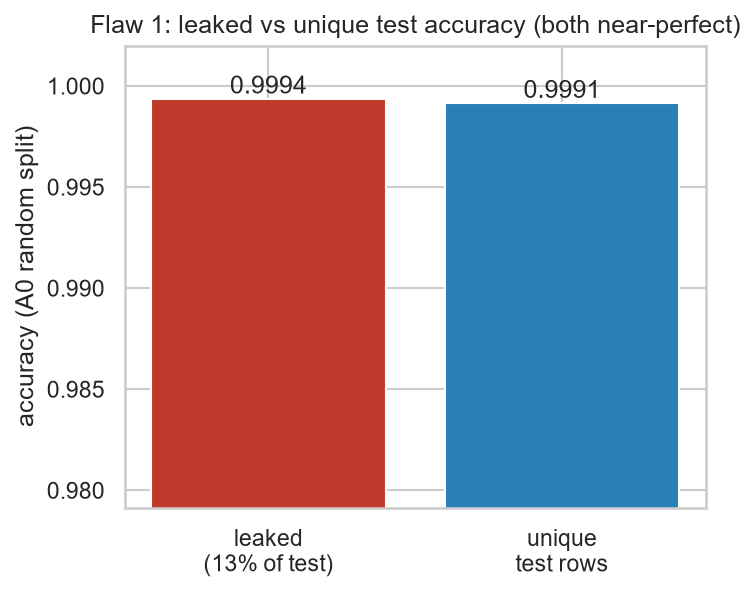
\includegraphics[width=0.55\textwidth]{07b_leakage_decomposition.png}
\caption{Leakage decomposition of the random split. Leaked (duplicated) and unique test
rows are classified with near-identical, near-perfect accuracy: the inflated headline does
not come from duplicate memorisation.}
\label{fig:leakage}
\end{figure}

\subsubsection*{Flaw 2 --- evaluation methodology: random vs.\ temporal split.}
A random split over a joint file mixes traffic from all days into both train and test.
Because CICIDS2017's attacks are day-segregated, this guarantees that every attack
\emph{type} is present in both partitions --- an \emph{in-distribution} test. A deployed IDS,
by contrast, is trained on past traffic and must detect \emph{future} (possibly novel)
attacks. We therefore evaluate honestly (Strategy B0): deduplicate, then split temporally
(train Monday--Thursday, test Friday), scale on train only, and balance the training set with
class-capped multiclass SMOTE before binarising.

The result is decisive (Figure~\ref{fig:split}): macro-F1 falls from $0.9984$ (random,
deduped) to $\mathbf{0.4883}$ (temporal), with accuracy $0.6764$, MCC $0.2541$, and
ROC-AUC $0.7735$. The \textbf{total gap from the source headline is
$0.9987 - 0.4883 = 0.5104$ (51.0 percentage points)}. The cause is unambiguous: 100\% of
Friday's attack flows (DDoS, PortScan, Botnet) belong to classes that never appear in
Monday--Thursday training. Per-attack-type recall on Friday confirms the collapse ---
DDoS $0.168$ (partial transfer from the seen DoS family), PortScan $0.001$, Botnet $0.000$.
Strategy B is thus effectively a near-zero-day generalisation test, and the random split was
hiding this entirely.

\begin{figure}[H]
\centering
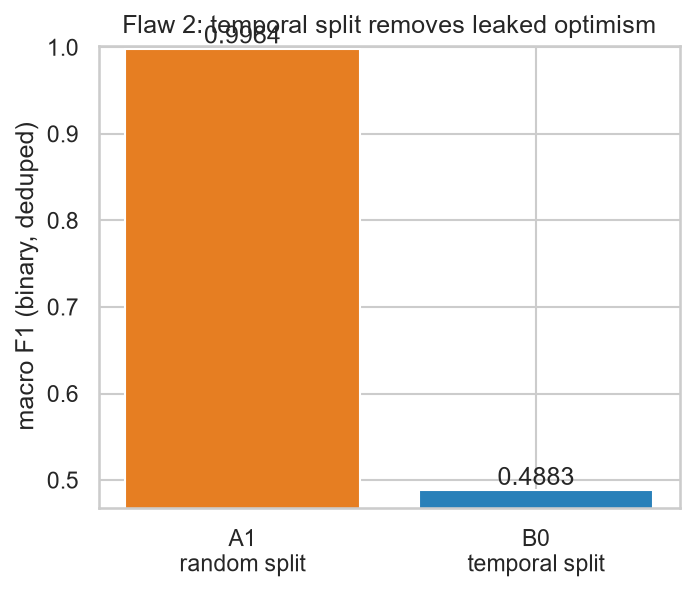
\includegraphics[width=0.5\textwidth]{08_split_impact_bar.png}
\caption{Binary macro-F1 under a random split vs.\ an honest temporal split. The 51-pp gap
is the optimism removed by respecting the temporal order of attacks.}
\label{fig:split}
\end{figure}

\subsubsection*{Flaw 3 --- a macro average hides rare-class failure.}
Reporting a single macro-F1 on a dataset that mixes 230k-sample classes with 11-sample
classes is statistically misleading. Using a stratified deduped multiclass model, the rare
classes have only 2--7 test samples each: Heartbleed recall $1.000$ (support $2$),
Infiltration $0.714$ (support $7$), SQL Injection $0.250$ (support $4$). These numbers are
\emph{un-evaluable}: any apparent ``hit'' is a memorised near-duplicate, and a single
aggregate number conceals that rare-but-dangerous attacks cannot be assessed at all.

\subsection{Are the conclusions justified? Verdict table}
\begin{table}[H]
\centering
\small
\begin{tabular}{>{\raggedright\arraybackslash}p{4.3cm} >{\raggedright\arraybackslash}p{3.6cm} >{\raggedright\arraybackslash}p{4.1cm} c}
\toprule
\textbf{Source claim} & \textbf{Our test} & \textbf{Our result} & \textbf{Supported?}\\
\midrule
F1 $\approx 0.999$ (their method) & raw + random split & A0 F1 $=0.999$ & Yes (reproduced)\\
0.999 holds after dedup & deduped + random split & A1 F1 $=0.998$ & Yes; leakage hidden\\
0.999 holds in deployment & deduped + temporal split & B0 F1 $=0.488$, MCC $0.254$ & \textbf{No}\\
Effective on all attack types & per-class recall & PortScan/Botnet recall $\approx 0$; rare classes un-evaluable & \textbf{No}\\
\bottomrule
\end{tabular}
\caption{Claim-by-claim verdict. The headline reproduces, but every claim about
\emph{generalisation} fails under sound evaluation.}
\end{table}

\textbf{Limitations of the source.} The paper (i) does not mention deduplication;
(ii) uses a random split on temporally-structured data; (iii) reports only an aggregate
metric, with no per-class breakdown for rare attacks; and (iv) reports no confidence
intervals or temporal robustness analysis. None of these are fatal individually, but together
they make the $0.999$ headline an in-distribution memorisation score rather than evidence of
a usable detector.

% =====================================================================
\section{Exploratory Data Analysis}
% =====================================================================
Before modelling, we explored the data to motivate every downstream decision.

\paragraph{Class imbalance and its real-world meaning.}
BENIGN traffic is $80.3\%$ of flows; the binary attack rate is $19.68\%$
(Figure~\ref{fig:classdist}). In a real network the benign fraction is usually \emph{higher}
still, so the imbalance is realistic in direction but the attack prevalence here is inflated by
the controlled capture. Imbalance means accuracy is an unreliable headline and motivates
recall-aware metrics (MCC, F$_\beta$) and resampling (SMOTE) on the training split only. The
source did not discuss imbalance handling.

\begin{figure}[H]
\centering
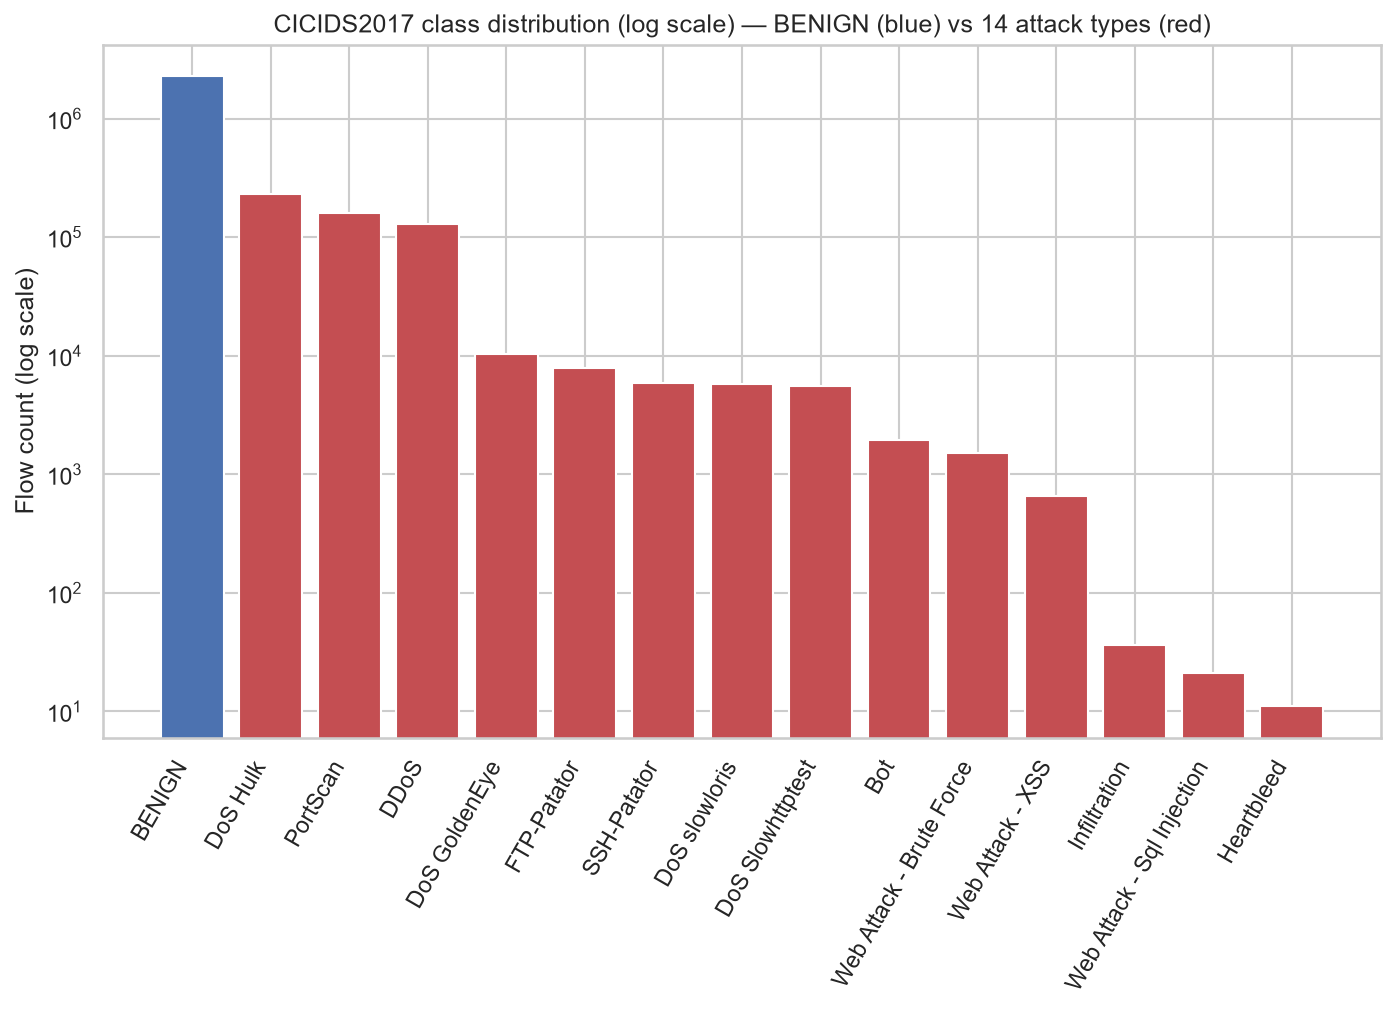
\includegraphics[width=0.7\textwidth]{01_class_distribution.png}
\caption{Class distribution (log scale). BENIGN dominates; rare attacks such as Heartbleed,
SQL Injection, and Infiltration have a handful of samples each.}
\label{fig:classdist}
\end{figure}

\paragraph{Temporal structure.}
Attacks are segregated by day (Figure~\ref{fig:byday}): this is the empirical basis for the
temporal-split critique. A data-driven cross-tab corrected the assumed mapping (Botnet, DDoS,
and PortScan are Friday phenomena). Because no clean temporal split can share attack
\emph{types} between train and test, Strategy B is necessarily a cross-attack-type test.

\begin{figure}[H]
\centering
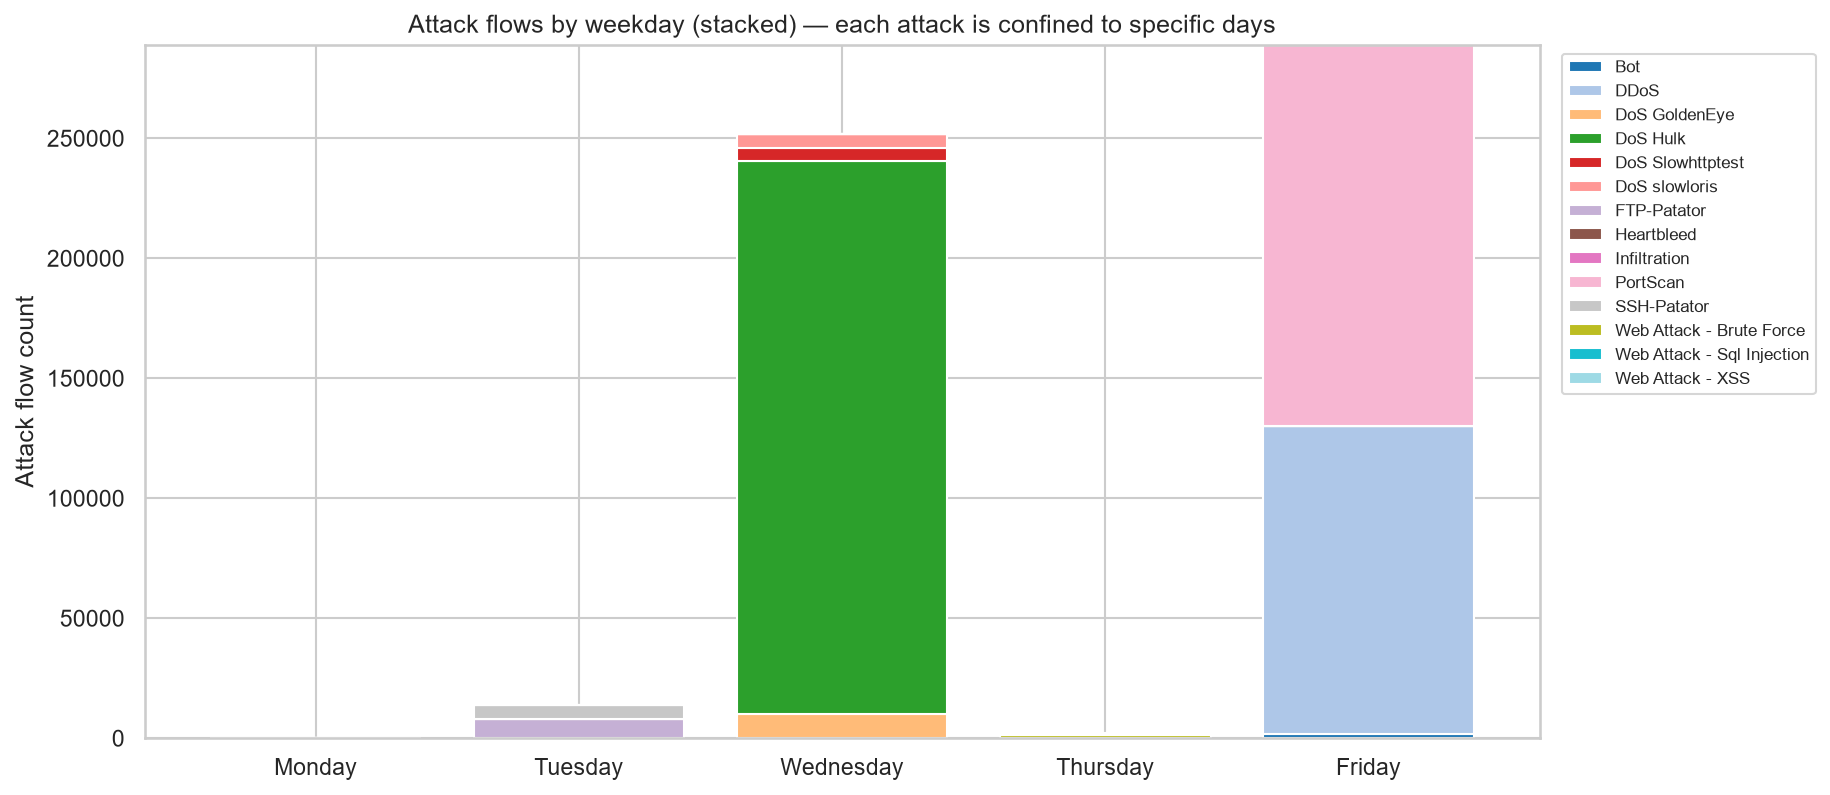
\includegraphics[width=0.7\textwidth]{02_attacks_by_day.png}
\caption{Attack composition by weekday. Each attack family is concentrated on specific days,
so a random split leaks attack-type membership across train and test.}
\label{fig:byday}
\end{figure}

\paragraph{Quality issues, distributions, and correlation.}
We found 4{,}376 \texttt{Inf} cells (in \texttt{Flow Bytes/s} and \texttt{Flow Packets/s},
a known CICFlowMeter artifact~\cite{engelen2021}), leading/trailing whitespace in column
names, a duplicated \texttt{Fwd Header Length.1} column, and 8 zero-variance columns. Most
features are heavily right-skewed (52 of 78 features have skewness $>3$), motivating a
\texttt{log1p} transform. For redundancy we used \textbf{Spearman} rank correlation rather
than Pearson, because the features are non-normal and outlier-heavy and we care about
monotonic (not strictly linear) association; Spearman is $O(n\log n)$ and robust to outliers,
whereas Kendall is prohibitively expensive on millions of rows. Many feature pairs exceed
$|r|>0.95$ (e.g.\ Subflow $\approx$ Total byte counts, segment-size $\approx$ packet-length
families), which we prune in feature engineering.

% =====================================================================
\section{Feature Engineering Analysis}
% =====================================================================
\paragraph{Was feature engineering performed, and which features were used?}
The raw data has 78 numeric flow features after dropping the day/label tags. We engineered a
40-feature matrix through the steps below; the binary label is
\texttt{(Label\,$\neq$\,BENIGN)} and the multiclass label is a 15-class encoding.

\paragraph{Transformations and their rationale.}
\begin{itemize}[leftmargin=1.4em,itemsep=2pt]
\item \textbf{Cleaning:} \texttt{Inf}$\rightarrow$\texttt{NaN} (CICFlowMeter artifact), column
whitespace stripping, label-encoding fixes for a non-UTF-8 dash in web-attack labels.
\item \textbf{Structural removal:} dropped the duplicated \texttt{Fwd Header Length.1} column
and 8 zero-variance columns (no information, pure noise/dimensionality).
\item \textbf{Log transform:} \texttt{log1p} applied to 23 right-skewed non-negative features
(7 skewed-but-negative features excluded). Skew $>3$ degrades distance/variance-based steps;
\texttt{log1p} is stateless, so applying it per split cannot leak.
\item \textbf{Scaling:} \texttt{StandardScaler} \emph{fit on the training split only}, then
applied to test --- the canonical no-leakage protocol.
\item \textbf{Encoding:} the only categorical is the target, handled with
\texttt{LabelEncoder}; features are already numeric, so no one-hot encoding is needed.
\item \textbf{Resampling:} class-capped multiclass SMOTE on the training split only
(interpolating within attack families, excluding ultra-rare classes), then binarised ---
never on combined data, to avoid optimistic leakage.
\end{itemize}

\paragraph{Redundancy: spotting and tackling it.}
We spotted redundancy via the Spearman matrix and pruned all features in a correlated pair
(over the full candidate set, $|r|>0.95$): 29 features removed, taking the matrix from
78 to \textbf{40} features. This is heavier pruning than a naive estimate because CICIDS2017
encodes the same quantity many ways (Subflow vs.\ Total, segment-size vs.\ packet length,
Active-time statistics). Redundant collinear features add variance and obscure importance
without adding signal.

\paragraph{Was the process meaningful, and what could improve it?}
Mathematically, removing collinear and zero-variance features reduces variance and improves
interpretability; in cybersecurity terms, the surviving features (flow durations, inter-arrival
times, packet-length statistics, flag counts) are the behavioural fingerprints that separate
scripted attacks from human traffic. Potential additions: entropy of destination ports,
windowed connection-rate features per source IP, and payload-derived signals --- none of which
the flow-only feature set captures, and which would likely help with novel attacks.

% =====================================================================
\section{Reproducibility Analysis}
% =====================================================================
\begin{itemize}[leftmargin=1.4em,itemsep=2pt]
\item \textbf{Can the code be executed?} Yes. Our notebook runs end-to-end via
\texttt{nbconvert --execute} on the full 2.83M-row dataset with zero errors and zero warnings,
producing all 16 figures and the metrics export.
\item \textbf{Are files and dependencies available?} Yes. Dependencies are pinned with
\texttt{uv} (\texttt{pyproject.toml} + \texttt{uv.lock}); the dataset is the public Kaggle
mirror of CICIDS2017, documented in the README and \texttt{references/}.
\item \textbf{Hidden preprocessing?} For \emph{the source}: yes --- deduplication is not
mentioned and the split strategy is under-specified, which is precisely what allows the
inflated headline. For \emph{our work}: no --- every step is an explicit, commented cell.
\item \textbf{Overall.} The source is only \emph{partially} reproducible: it uses Weka with no
public code, so the exact pipeline must be inferred. Our Python re-implementation is fully
reproducible (fixed seeds, no leakage, conventional commits, \texttt{ruff}-clean), which is
itself a contribution: it makes the claim falsifiable.
\item \textbf{Engineering.} The reusable core is factored into a tested package
\texttt{src/ids\_critique/} (\texttt{data} / \texttt{features} / \texttt{evaluate} /
\texttt{critique}) with \textbf{16 passing \texttt{pytest} unit tests}; the environment is
pinned via \texttt{uv.lock} (Python 3.12, scikit-learn 1.9, XGBoost 3.3, imbalanced-learn 0.14).
Full version and command details are in Appendix~A.
\end{itemize}

% =====================================================================
\section{Experimental Results}
% =====================================================================
\subsection{Experiments and modifications}
We ran five experiments: \textbf{A0} (raw + random, the source method), \textbf{A1}
(deduped + random, isolating Flaw~1), \textbf{B0} (deduped + temporal + SMOTE, the honest
protocol), \textbf{Bm} (deduped stratified multiclass, for per-class recall), and two honest
alternatives --- \textbf{XGBoost} and an unsupervised \textbf{Isolation Forest}. Our key
modification relative to the source is the honest temporal split plus the full,
recall-aware metric suite.

\subsection{Model training and comparison}
All supervised models share the temporal protocol so the comparison is fair
(Figure~\ref{fig:modelcmp}). Under that honest split, no supervised model is usable:
XGBoost reaches macro-F1 $0.4972$ (MCC $0.2670$, ROC-AUC $0.7425$), marginally above the
Random Forest ($0.4883$). The unsupervised Isolation Forest --- trained on benign flows only,
so it does not depend on having seen an attack class --- achieves the best honest
\emph{attack recall} ($0.328$) and binary F1 ($0.547$), precisely because it treats Friday's
novel attacks as anomalies rather than memorised classes.

\begin{table}[H]
\centering\footnotesize
\setlength{\tabcolsep}{3.4pt}
\begin{tabular}{l c c c c c c c}
\toprule
\textbf{Model (protocol)} & \textbf{macro-F1} & \textbf{prec.} & \textbf{recall} & \textbf{F1$_+$} & \textbf{F$_2$} & \textbf{MCC} & \textbf{AUC}\\
\midrule
RF --- A0 (raw + random, \emph{source}) & \textbf{0.9987} & 0.997 & 0.999 & 0.998 & 0.999 & 0.997 & 1.000\\
RF --- A1 (deduped + random) & 0.9984 & 0.997 & 0.998 & 0.997 & 0.998 & 0.997 & 1.000\\
\midrule
RF --- B0 (deduped + temporal) & \textbf{0.4883} & 0.997 & 0.098 & 0.178 & 0.119 & 0.254 & 0.774\\
XGBoost --- B1 (deduped + temporal) & 0.4972 & 0.997 & 0.108 & 0.194 & 0.131 & 0.267 & 0.742\\
Isolation Forest --- B2 (unsupervised) & 0.5473 & 0.443 & 0.328 & 0.377 & 0.346 & 0.106 & 0.740\\
\bottomrule
\end{tabular}
\caption{Full metric suite. \emph{macro-F1} averages both classes (the source's headline); the
remaining columns are positive-class (attack) metrics. The honest-protocol rows (B$\ast$) expose
the recall collapse that accuracy and the macro headline hide --- note B0/B1's high precision
(0.997) but $\approx$0.10 recall: they almost never false-alarm, yet miss $\approx$90\% of attacks.}
\end{table}

\begin{table}[H]
\centering\small
\begin{tabular}{l r c l}
\toprule
\textbf{Friday attack type} & \textbf{flows} & \textbf{recall (B0)} & \textbf{seen in training?}\\
\midrule
DDoS & 128{,}014 & 0.168 & no (partial transfer from DoS family)\\
PortScan & 90{,}694 & 0.001 & no\\
Botnet & 1{,}948 & 0.000 & no\\
\bottomrule
\end{tabular}
\caption{Per-attack-type recall on the Friday temporal test (B0). 100\% of the day's attack
flows belong to classes unseen in Mon--Thu training, which is why recall collapses.}
\end{table}

\begin{figure}[H]
\centering
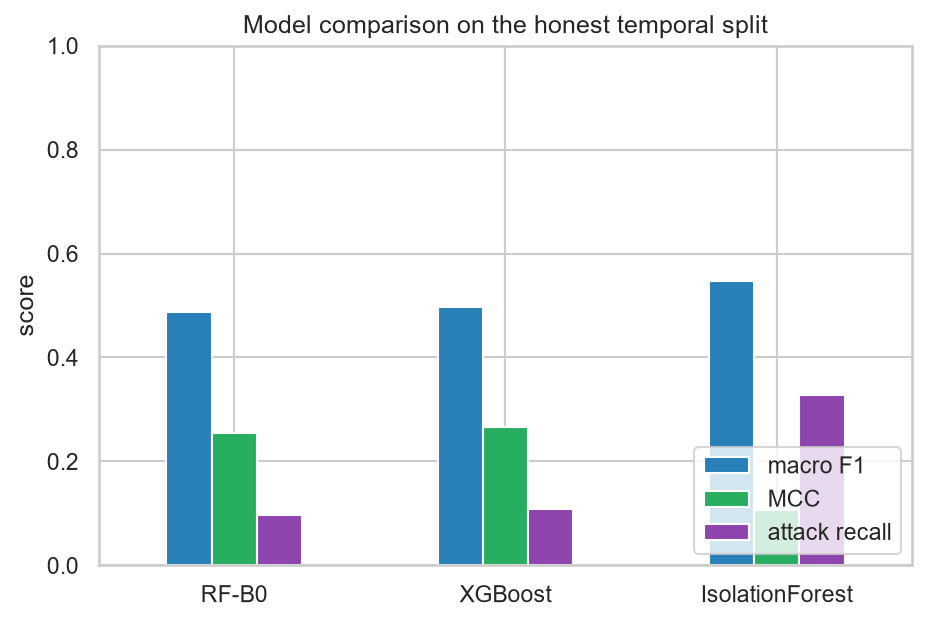
\includegraphics[width=0.7\textwidth]{14_model_comparison_bar.png}
\caption{Model comparison on the honest temporal split (F1 / MCC / attack recall). All models
are far from the inflated $0.999$; the unsupervised model wins on attack recall.}
\label{fig:modelcmp}
\end{figure}

\subsection{Evaluation metrics: definitions and why they matter for IDS}
We deliberately go beyond the source's single macro-F1. For each metric we give its meaning
and its cybersecurity interpretation; the false-positive (FP) vs.\ false-negative (FN)
trade-off is what makes the choice non-trivial.
\begin{itemize}[leftmargin=1.4em,itemsep=2pt]
\item \textbf{Accuracy} $=\frac{TP+TN}{N}$. \emph{Misleading here}: an ``always BENIGN''
classifier scores $\approx0.83$ on the Friday test while detecting nothing. We report it only
to demonstrate this trap.
\item \textbf{Precision} $=\frac{TP}{TP+FP}$. The fraction of alerts that are real ---
governs SOC \emph{alert fatigue}. Low precision floods analysts with false alarms.
\item \textbf{Recall} $=\frac{TP}{TP+FN}$. The fraction of attacks caught --- the most
critical IDS metric, since each FN is an undetected intrusion.
\item \textbf{F1} $=\frac{2\,PR}{P+R}$ and \textbf{F$_\beta$} ($\beta{=}2$), which weights
recall higher because missing an attack costs more than a false alarm.
\item \textbf{MCC} (Matthews correlation, range $[-1,1]$): robust to imbalance and our
preferred single number; B0's MCC $=0.254$ exposes that the model is only weakly better than
chance, which accuracy ($0.676$) hides.
\item \textbf{ROC-AUC / PR-AUC}: threshold-free ranking quality. Under heavy imbalance the
precision--recall curve (Figure~\ref{fig:pr}) is more informative than ROC because true
negatives dominate.
\item \textbf{Confusion matrix} (per class, Figure~\ref{fig:confusion}): the only view that
reveals \emph{which} classes fail.
\end{itemize}

\begin{figure}[H]
\centering
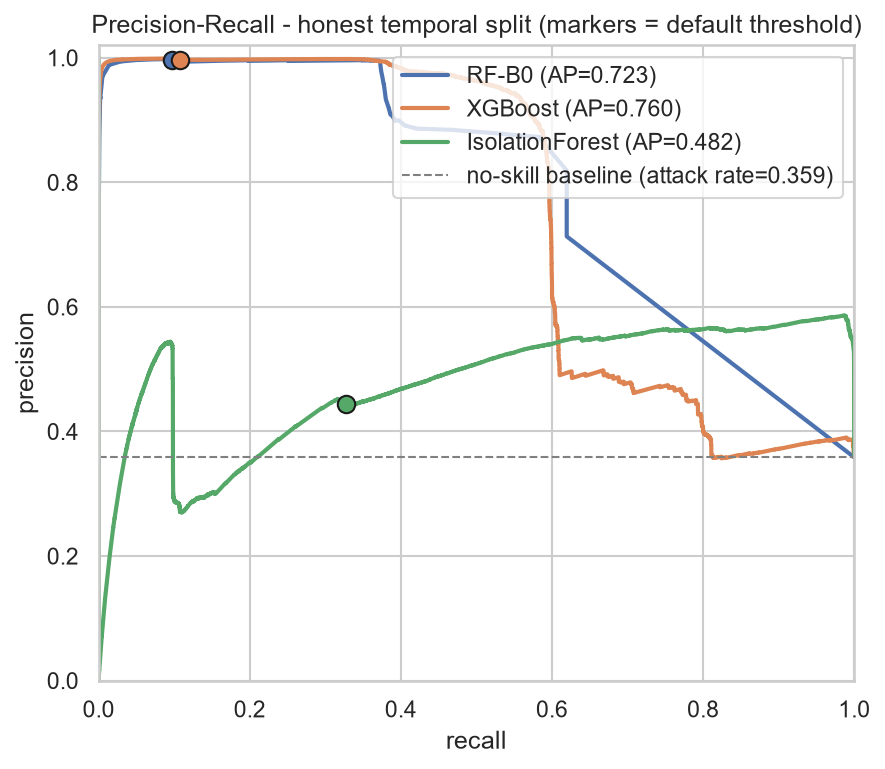
\includegraphics[width=0.62\textwidth]{13_pr_curve_threshold.png}
\caption{Precision--recall curves on the honest temporal split; markers show each model's
default-threshold operating point against the no-skill baseline.}
\label{fig:pr}
\end{figure}

% =====================================================================
\section{Error Analysis}
% =====================================================================
\paragraph{Failures and their patterns.}
On the Friday temporal test, the Random Forest's false negatives are dominated by the novel
attack families: PortScan ($99.9\%$ missed) and Botnet ($100\%$ missed), with DDoS partially
caught ($16.8\%$ recall) thanks to transfer from the seen DoS family. The errors are
\emph{structural}, not noise: 100\% of Friday's attacks are classes unseen in training, so the
model has no learned signature for them. The row-normalised multiclass confusion matrix
(Figure~\ref{fig:confusion}) shows the rare-class rows going dark --- the visual signature of
Flaw~3.

\begin{figure}[H]
\centering
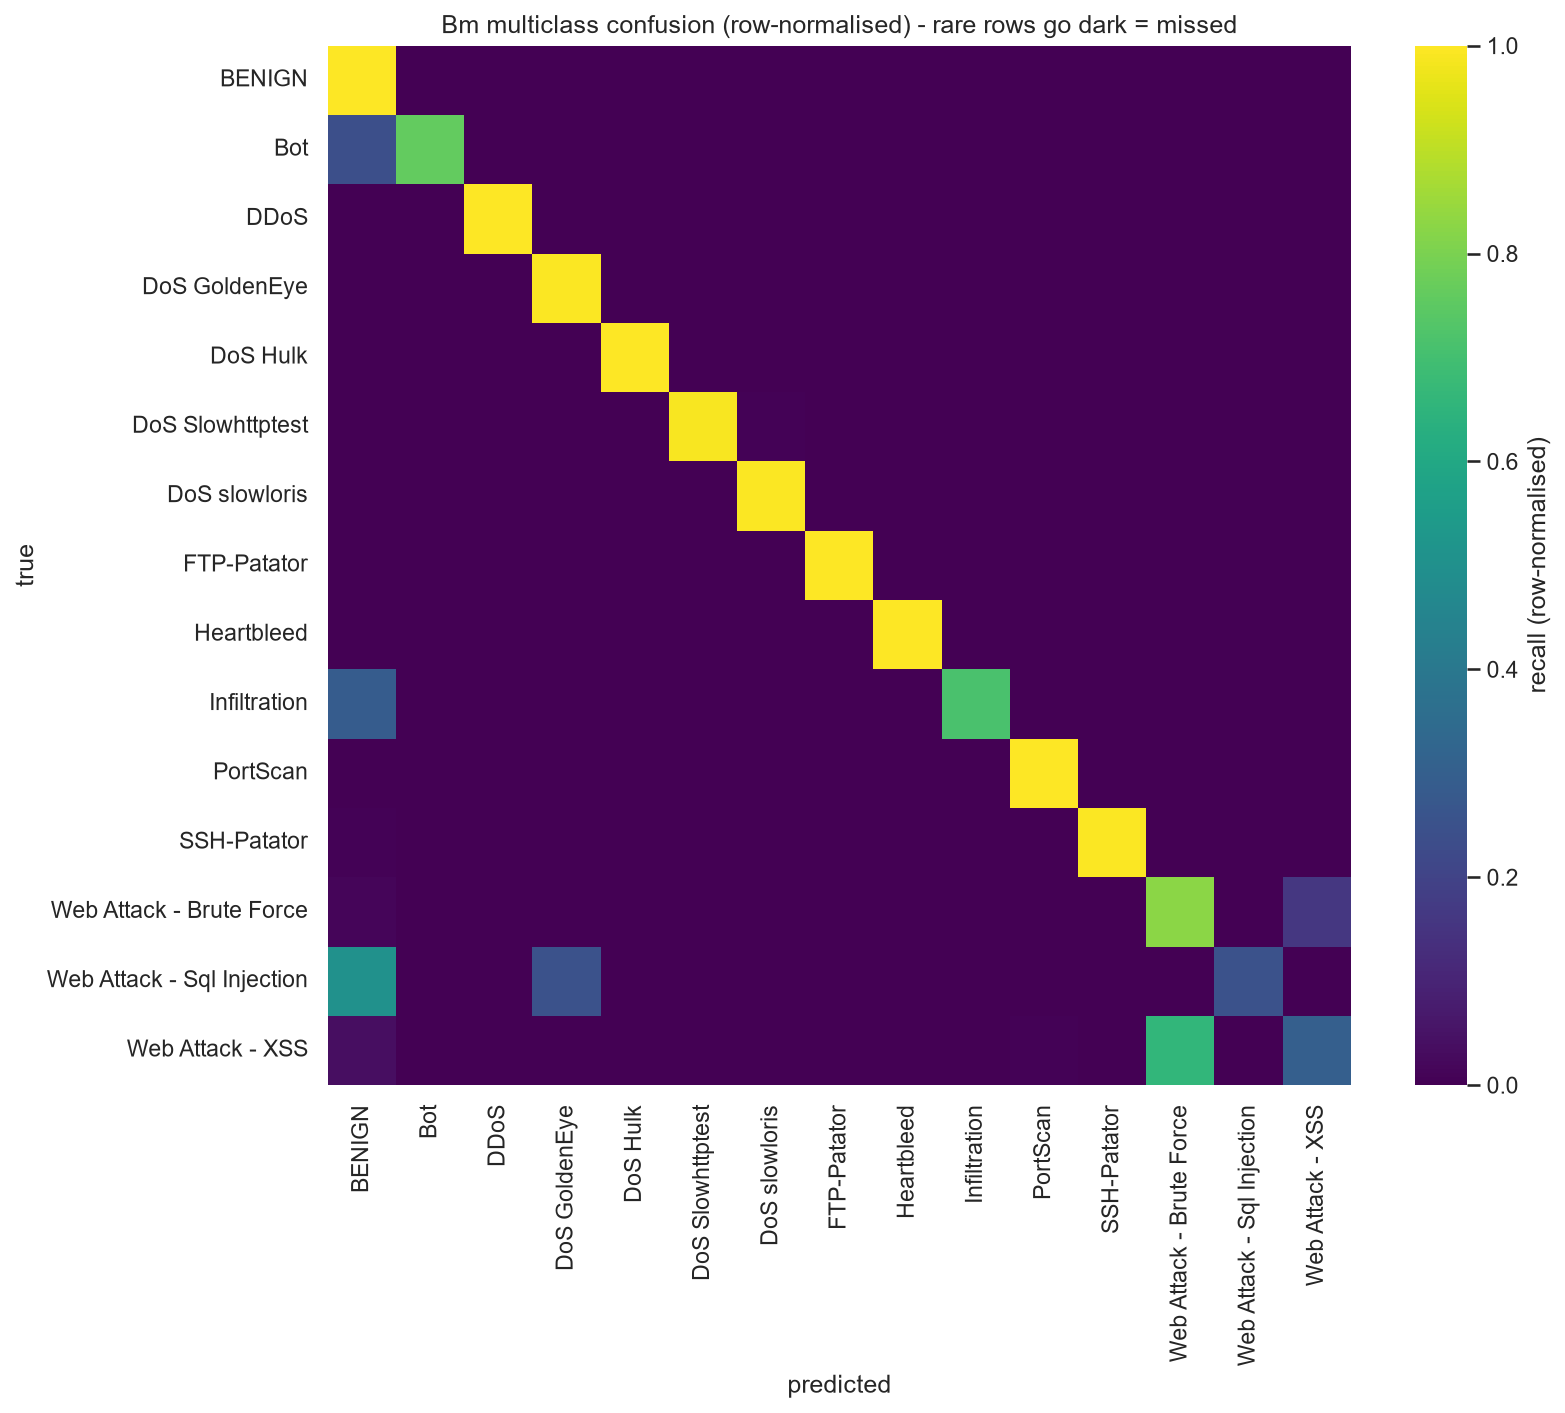
\includegraphics[width=0.78\textwidth]{10_confusion_strategyB.png}
\caption{Row-normalised multiclass confusion matrix. Bright diagonal cells are recovered
classes; dark rare-attack rows are systematically missed.}
\label{fig:confusion}
\end{figure}

\begin{figure}[H]
\centering
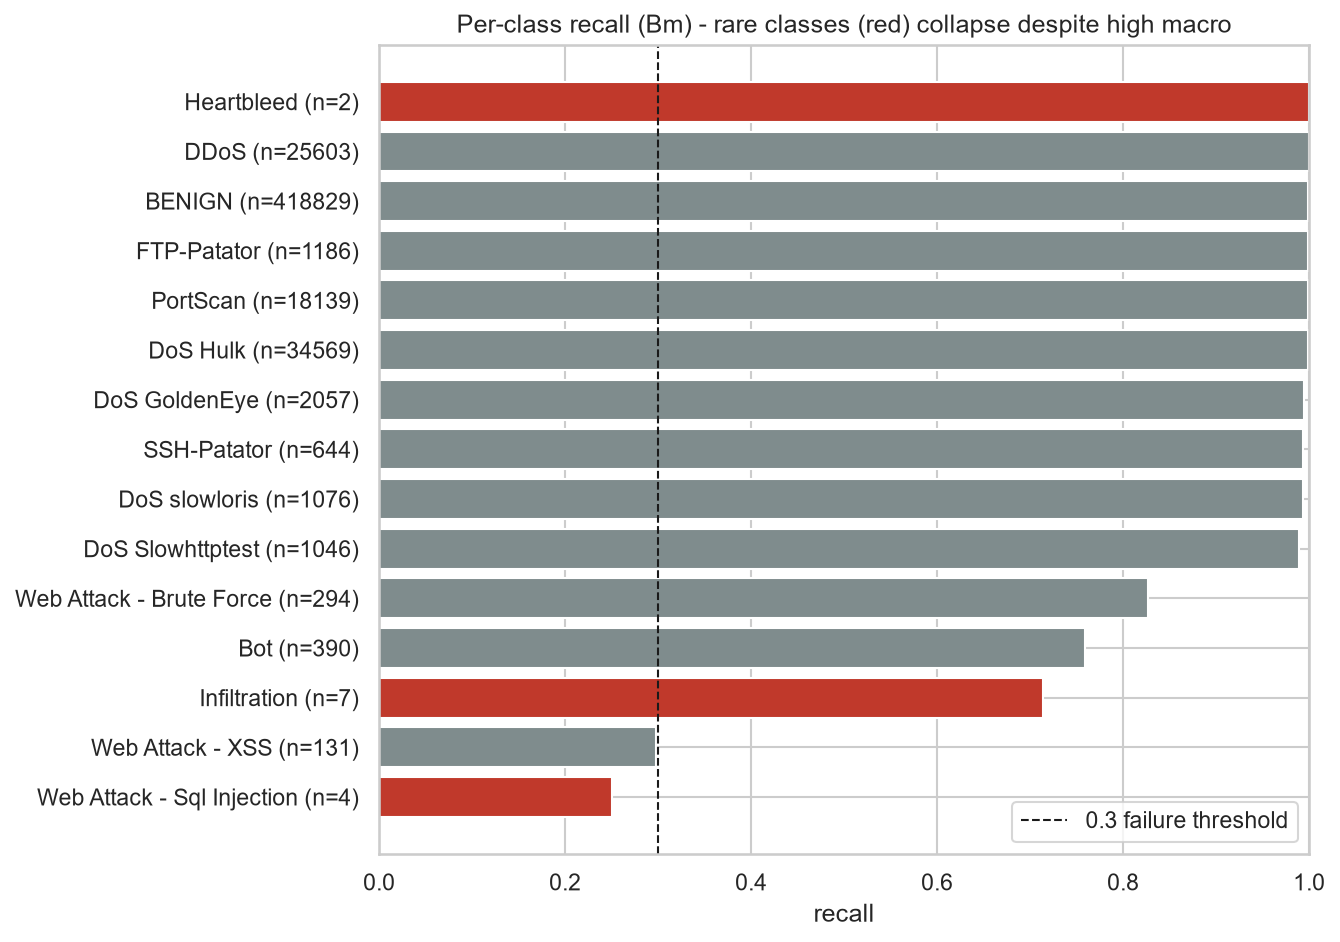
\includegraphics[width=0.7\textwidth]{11_perclass_recall_bar.png}
\caption{Per-class recall (rare classes in red). High macro/aggregate numbers coexist with
near-zero recall on dangerous, rare attacks.}
\label{fig:perclass}
\end{figure}

\paragraph{Cybersecurity implication and the FP/FN trade-off.}
Read as one day of traffic, the honest model raises a non-trivial alert queue while still
missing the majority of the day's attacks. In SOC terms, an analyst trusting the source's
$0.999$ would expect near-total coverage; in reality the detector misses most novel attacks.
Because a missed intrusion (FN) is far costlier than a false alarm (FP), the right operating
point sits high on the recall axis --- which on this honest split means accepting poor
precision, or (better) using anomaly detection and frequent retraining rather than a
supervised classifier alone.

\begin{table}[H]
\centering\small
\begin{tabular}{l r}
\toprule
\textbf{Friday (one day of traffic), honest RF-B0} & \textbf{count}\\
\midrule
Flows processed & 703{,}245\\
Real attacks present & 220{,}656\\
Alerts raised & 21{,}636\\
\quad of which false alarms & 65 \;(0.3\% of the alert queue)\\
Real attacks missed (false negatives) & 199{,}085 \;(90.2\% of attacks)\\
\bottomrule
\end{tabular}
\caption{SOC cost on a single day. The honest detector barely false-alarms (high precision) yet
misses 90\% of the day's attacks --- the operational opposite of the ``0.999'' impression.}
\end{table}

% =====================================================================
\section{Conclusions}
% =====================================================================
\paragraph{Key findings.} (1) The $0.999$ headline reproduces under the source's protocol but
is an artifact of in-distribution memorisation. (2) Duplicate leakage, contrary to the common
narrative, is \emph{not} the inflation lever here ($+0.03$~pp); attack-type overlap in a random
split is. (3) An honest temporal split drops macro-F1 by $51$~pp because Friday's attacks are
novel. (4) Aggregate metrics hide that rare classes are un-evaluable.

\paragraph{Lessons learned.} Evaluation design dominates model choice on this dataset:
the same Random Forest scores $0.999$ or $0.488$ depending only on how the split is made.
Intellectual honesty (reporting the duplicate null result) made the critique stronger, not
weaker.

\paragraph{Strengths and weaknesses of the source.} \emph{Strengths}: a broad, peer-reviewed
model comparison on a standard dataset. \emph{Weaknesses}: no deduplication, a leakage-prone
random split on temporally-structured data, and aggregate-only metrics.

\paragraph{Future improvements.} Temporal or attack-type-disjoint evaluation; deduplication
with leakage reporting; per-class recall with explicit handling of un-evaluable classes;
recall-aware metrics (MCC, F$_\beta$, PR-AUC); anomaly detection for novel attacks; and
periodic retraining to handle concept drift.

% =====================================================================
\section{Executive Summary}
% =====================================================================
\textbf{Problem.} Flow-based network intrusion detection on CICIDS2017 (2.83M flows,
$\approx 80\%$ benign, 14 attack types over Mon--Fri).

\textbf{Source.} Rodr\'iguez et al.\ (2022, \emph{Sensors} MDPI) report Random-Forest
F1 $>0.999$ using a random split over all days concatenated, no deduplication, and a
macro-F1-only headline.

\textbf{Methodology of our study.} We rebuilt their pipeline in Python/scikit-learn and ran it
three ways --- A0 (their protocol), A1 (their protocol + deduplication), B0 (honest temporal
split) --- plus XGBoost and an unsupervised Isolation Forest, with a full recall-aware metric
suite and per-class analysis.

\textbf{Main findings.} A0 reproduces F1 $=0.9987$; deduplication changes it by only
$+0.03$~pp; the honest temporal split collapses macro-F1 to $0.4883$ (MCC $0.254$), a
$51$-pp drop driven by 100\% novel Friday attack classes; rare attacks have 2--7 evaluable
samples and are effectively undetected.

\textbf{Were the author's claims supported?} The number is reproducible, but the implied claim
of a generalising detector is \textbf{not supported}.

\textbf{Most important insight.} On day-segregated data, a random split measures memorisation,
not detection; evaluation design, not the model, produces the $0.999$.

\textbf{Do we recommend reusing this approach on similar problems?} \textbf{No} --- not without
temporal/novel-attack-aware evaluation, deduplication with leakage reporting, per-class recall,
and recall-aware metrics. With those corrections the \emph{workflow} is sound; the original
\emph{evaluation} is not.

\textbf{Final conclusion.} The headline is an evaluation artifact; the honest performance is
modest, and the project demonstrates why methodological rigor matters more than a single
impressive number --- consistent with Engelen et al.\ (2021)~\cite{engelen2021} and
Lanvin et al.\ (2022)~\cite{lanvin2022}.

% =====================================================================
\section{Summing It Up}
% =====================================================================
This project critically evaluated a peer-reviewed claim that Random Forest attains
F1 $>0.999$ for flow-based intrusion detection on CICIDS2017. We reproduced the number under
the original protocol, then demonstrated --- with our own controlled experiments --- that it
does not survive sound evaluation: deduplication leaves it essentially unchanged (so the
common ``duplicate leakage'' explanation is, here, a footnote), an honest temporal split
removes $51$ percentage points because the test day's attacks are novel, and aggregate metrics
conceal that rare attacks cannot be evaluated. The objective was not to critique our own
implementation but to assess the validity of the original work; our verdict is that the
author's conclusions, while reproducible, are \emph{not justified} as evidence of a deployable
detector. A successful outcome here is the rigorous, honest analysis itself --- whether or not
the original claim is confirmed.

% =====================================================================
\appendix

\section{Reproducibility \& Environment}
The full study runs from a pinned environment with one command; all randomness is fixed via
\texttt{RANDOM\_STATE = 42}.

\begin{table}[H]
\centering\small
\begin{tabular}{l l}
\toprule
\textbf{Item} & \textbf{Value}\\
\midrule
Python & 3.12\\
Environment manager & \texttt{uv} (pinned in \texttt{uv.lock})\\
Core libraries & scikit-learn 1.9, XGBoost 3.3, imbalanced-learn 0.14, pandas, numpy\\
Notebook execution & \texttt{jupyter nbconvert --execute} --- 0 errors, 0 warnings, 16 figures\\
Linting & \texttt{ruff check .} --- clean\\
Unit tests & \texttt{pytest} --- 16 passing (\texttt{tests/}, dataset-independent)\\
Report build & MiKTeX / \texttt{pdflatex} (this document)\\
Repository & \texttt{github.com/eyalsht/ids-cicids2017-critique} (public)\\
\bottomrule
\end{tabular}
\caption{Environment and reproducibility summary.}
\end{table}

\noindent Reusable logic is factored into a tested package and mirrors the notebook's helpers:
\begin{itemize}[leftmargin=1.4em,itemsep=1pt]
\item \texttt{src/ids\_critique/data.py} --- weekday parsing, whitespace/Inf cleaning, duplicate counting.
\item \texttt{src/ids\_critique/features.py} --- skew detection, \texttt{log1p}, correlation pruning.
\item \texttt{src/ids\_critique/evaluate.py} --- the IDS metric suite.
\item \texttt{src/ids\_critique/critique.py} --- the flaw deltas (inflation, temporal drop, novel-class share).
\end{itemize}

\section{Rubric Traceability}
\begin{table}[H]
\centering\small
\begin{tabular}{l c l}
\toprule
\textbf{Rubric component} & \textbf{Pts} & \textbf{Primary evidence}\\
\midrule
Problem Understanding \& Source Selection & 10 & \S1; README; \texttt{references/source\_article.md}\\
Summary Quality & 15 & \S1\\
\textbf{Critical Evaluation of Claims} & \textbf{20} & \S2 (three flaws, deltas, verdict table)\\
Feature Engineering Analysis & 10 & \S4; notebook \S3; \texttt{features.py}\\
Exploratory Data Analysis & 15 & \S3; notebook \S2; Figures 3--4\\
Model Training \& Comparison & 15 & \S6; notebook \S4; Figures 7--8\\
Evaluation \& Error Analysis & 10 & \S6--\S7; notebook \S5--\S6\\
Code Quality \& Software Engineering & 5 & \texttt{src/}, \texttt{tests/}, \texttt{uv}, ruff-clean, fixed seeds\\
\bottomrule
\end{tabular}
\caption{Mapping of each grading-rubric component to its primary evidence in this submission.}
\end{table}

% =====================================================================
\begin{thebibliography}{9}
\bibitem{rodriguez2022}
M.~Rodr\'iguez, \'A.~Alesanco, L.~Mehavilla, and J.~Garc\'ia,
``Evaluation of Machine Learning Techniques for Traffic Flow-Based Intrusion Detection,''
\emph{Sensors}, vol.~22, no.~23, p.~9326, 2022. DOI: 10.3390/s22239326.

\bibitem{engelen2021}
G.~Engelen, V.~Rimmer, and W.~Joosen,
``Troubleshooting an Intrusion Detection Dataset: the CICIDS2017 Case Study,''
\emph{2021 IEEE Security and Privacy Workshops (SPW)}, pp.~7--12, 2021.
DOI: 10.1109/SPW53761.2021.00009.

\bibitem{lanvin2022}
M.~Lanvin, P.-F.~Gimenez, Y.~Han, F.~Majorczyk, L.~M\'e, and E.~Totel,
``Errors in the CICIDS2017 Dataset and the Significant Differences in Detection Performances
It Makes,'' \emph{17th International Conference on Risks and Security of Internet and Systems
(CRiSIS)}, 2022.

\bibitem{sharafaldin2018}
I.~Sharafaldin, A.~H.~Lashkari, and A.~A.~Ghorbani,
``Toward Generating a New Intrusion Detection Dataset and Intrusion Traffic
Characterization,'' \emph{4th International Conference on Information Systems Security and
Privacy (ICISSP)}, pp.~108--116, 2018.
\end{thebibliography}

\end{document}
